\PassOptionsToPackage{table}{xcolor}
\documentclass[10pt]{beamer}
\usepackage[english]{babel}

\usetheme{metropolis}
\usepackage{smartdiagram}
\usepackage{listings}
\usepackage{booktabs}
\usepackage[scale=2]{ccicons}%creative commons
\setbeamercovered{transparent}%invisible by default
\usepackage{array}
\newcolumntype{L}[1]{>{\raggedright\let\newline\\\arraybackslash\hspace{0pt}}m{#1}}
\newcolumntype{C}[1]{>{\centering\let\newline\\\arraybackslash\hspace{0pt}}m{#1}}
\newcolumntype{R}[1]{>{\raggedleft\let\newline\\\arraybackslash\hspace{0pt}}m{#1}}

\usepackage{pgfplots}
\usepgfplotslibrary{dateplot}
\usepackage{tikz}
\usepackage{tikz-uml}
\usetikzlibrary{positioning,chains,fit,shapes,calc}

\newcommand{\mycomment}[1]{}
\usepackage{fancyvrb}
% *****************************************************************************
% Matematica 
% *****************************************************************************

%\usepackage{amssymb}
%\usepackage{mathtools}                    % Add support for cramped,
					  
%\usepackage[euler]{flexisym}
%\usepackage{breqn}                        % Breqn
%\makeatletter
%   \def\eqnumsize{\normalfont \Tf@font}      % Add support to Minion Pro
%\makeatother
%\setkeys{breqn}{labelprefix={eq:}}


%\usepackage{asymptote}
%\usepackage[loop, controls]{animate}

\graphicspath{{./}, {./Images/}}

\lstdefinelanguage{Kotlin}{
  keywords={package, as, typealias, this, super, val, var, fun, for, null, true, false, is, in, throw, return, break, continue, object, if, try, else, while, do, when, yield, typeof, yield, typeof, class, interface, enum, object, override, public, private, get, set, import, abstract, },
  keywordstyle=\color{blue}\bfseries,
  ndkeywords={@Deprecated, Int, Integer, Float, Double, String, Runnable, dynamic},
  ndkeywordstyle=\color{red}\bfseries,
  emph={println, return@, forEach,},
  emphstyle={\color{red}},
  identifierstyle=\color{black},
  sensitive=true,
  commentstyle=\color{gray}\ttfamily,
  comment=[l]{//},
  morecomment=[s]{/*}{*/},
  stringstyle=\color{gray}\ttfamily,
  morestring=[b]",
  morestring=[s]{"""*}{*"""},
}

\providecommand{\ie}{i.\,e.}
\providecommand{\Ie}{I.\,e.}
\providecommand{\eg}{e.\,g.}
\providecommand{\Eg}{E.\,g.} 

\metroset{block=fill}
\metroset{titleformat frame=smallcaps}

\title{Dependency injection made easy with Dagger2}
%\subtitle{and how it can help us building better reactive code}

\date{\today}
\author[A. Candolini]{Alessandro Candolini}
%\institute{Department of Physics, University of Trieste}
% \titlegraphic{\hfill\includegraphics[height=1.5cm]{logo/logo}}

\begin{document}

\maketitle

\begin{frame}{Agenda}
  \setbeamertemplate{section in toc}[sections numbered]
  \tableofcontents[hideallsubsections]
\end{frame}

\section{Dependency injection principles}
\begin{frame}[fragile]
	\frametitle{What is a dependency?}
		\begin{figure}
			\centering
\begin{tikzpicture}
\umlsimpleclass [minimum height=15ex,width=15ex] {A}
	\umlsimpleclass[x=4,width=5ex]{B}
\umlunicompo[geometry=|-|]{A}{B}
\end{tikzpicture}
		\end{figure}
\end{frame}
\begin{frame}[fragile]
%\begin{lstlisting}[language=java,basicstyle=\ttfamily,keywordstyle=\color{red}]
\begin{lstlisting}[language=Kotlin, basicstyle=\ttfamily]
/** Class A (the client) */
class A {
    // ....
    fun doSomething() {
        b.log("text")
    }
}

/** Class B (dependency/service) */
class B {
    fun log(text : String) {
    }
}
\end{lstlisting} 
\end{frame}
	\begin{frame}[fragile]
\begin{lstlisting}[language=Kotlin, basicstyle=\ttfamily]
// Option 1 - static methods 

class A {
    fun doSomething() {
        B.log("text") // <- static method
    }
}

class B {
    companion object {
        fun log(text: String) {
        }
    }
}
\end{lstlisting} 
	\end{frame}

	\begin{frame}
		Examples:
		\begin{itemize}
			\item Helper  classes
			\item Utils  classes
			\item Manager classes, etc\ldots
		\end{itemize}
	\end{frame}

	\begin{frame}[fragile]
		Drawbacks:
		\begin{itemize}
			\item $A$ not testable in isolation (integration test of $A$ \& $B$)
			\item $A$ \emph{strongly coupled} to $B$ (hardcoded dependency, no way to override/replace it) 
			\item Lack of encapsulation  (backdoor) 
			\item \emph{Hidden} dependency 
		\end{itemize}
	\end{frame}
	\begin{frame}[fragile]
		More Examples:
		\begin{itemize}
			\item \verb|Application.getStaticContext()|
			\item in order to move one class to a different module, you have to move ``hundreds`` of classes\ldots 
		\end{itemize}
	\end{frame}
\begin{frame}[fragile]
\begin{lstlisting}[language=Kotlin, basicstyle=\ttfamily]
// Option 2 - singletons

class A {
    fun doSomething() {
	B.log("text") // <- singleton
    }
}

object B {
    fun log(text: String) {
    }
}
\end{lstlisting} 
\end{frame}
\begin{frame}[fragile]
\begin{lstlisting}[language=Kotlin, basicstyle=\ttfamily]
// Option 3 - composition 

class A {
    private val b : B = B() // <-- instantiate
    
    fun doSomething() {
        b.log("text")
    }
}

class B {
    fun log(text: String) {
    }
}
\end{lstlisting} 
\end{frame}
	\begin{frame}[fragile]
		%\frametitle{Composition}
		\begin{figure}
			\centering
\begin{tikzpicture}
	\umlclass{A}{}{+ doSomething() : void}
	\umlclass [x=5, y=0] {B}{}{+ log(text : String) : void}
\umlunicompo{A}{B}
\end{tikzpicture}
		\end{figure}
			The \emph{life} of the child is completely controlled by the parent.
%\begin{tikzpicture}
%\umlsimpleclass [x=0,width=15ex] {A}
%\umlsimpleclass [ x=10ex, y=0] {B}
%\umlunicompo[geometry=|-|]{A}{B}
%\end{tikzpicture}
	\end{frame}
	\begin{frame}[fragile]
		Example:
		\begin{itemize}
			\item Custom views or adapters instantiating objects 
			\item \verb|Date date = new Date()| (imagine test today date) 
		\end{itemize}
	\end{frame}

	\begin{frame}[fragile]
		Drawbacks:
		\begin{itemize}
			\item $A$ is in charge of instantiating $B$ (additional responsibility)
			\item $A$ can't be tested in isolation (integratin test of $A$ and $B$ together) 
			\item $A$ is strongly coupled to $B$ (can't replace $B$ rom outside and/or in testing) 
		\end{itemize}
	\end{frame}
\begin{frame}[fragile]
\begin{lstlisting}[language=Kotlin, basicstyle=\ttfamily]
// Externalise the dependency 

class A(private val b : B) {
    fun doSomething() {
	b.log("text") 
    }
}

class B {
    fun log(text: String) {
    }
}
// 
val b : B = B()
val a : A = A(b) // <-- plug b
\end{lstlisting} 
\end{frame}

\plain{We can do even better\ldots}
\begin{frame}[fragile]
\begin{lstlisting}[language=Kotlin, basicstyle=\ttfamily]

class A(private val b : B) {
    fun doSomething() {
	b.log("text") 
    }
}

interface B {
    fun log(text: String);
}

class AmazingB : B {
    override fun log(text : String) {
    }
}
// 
val b : B = AmazingB()
val a : A = A(b)
\end{lstlisting} 
\end{frame}

\begin{frame}[fragile]
	Now we have:
	\begin{itemize}
		\item Full decoupling
		\item $A$ loosely coupled to $B$ ($A$ knows anything about $B$ but the contract) 
		\item Inversion of control%
			\footnote{Not yet actually\ldots We miss an ingredient}: it's no longer responsibility of $A$ to get its own dependencies 
	\end{itemize}
\end{frame}
\mycomment{
\begin{frame}[fragile]
\begin{lstlisting}[language=Kotlin, basicstyle=\ttfamily]
interface Transaction

interface Store { // repository/gateway pattern
    fun fetch(id : String) : Transaction
}

class UseCase(val store: Store) { /* .. */ }

\end{lstlisting} 
\end{frame}
\begin{frame}[fragile]
\begin{lstlisting}[language=Kotlin, basicstyle=\ttfamily]
class BaseStore : Store {
    override fun fetch(id : String): Transaction {/*...*/}
}

// Delegation pattern
class StoreA(val store: Store) : Store by store {
    override fun fetch(id : String): Transactions {
        /* do something */
    }
}

// Delegation pattern 
class StoreB(val store: Store) : Store by store {
    override fun fetch(id : String): Transactions {
        /* do something else */
    }
}
\end{lstlisting} 
\end{frame}
}
\begin{frame}[fragile]
	There is a problem:
\begin{lstlisting}[language=Kotlin, basicstyle=\ttfamily]
class C {
    fun qhdouwh() {
        val b = AmazingB() // <--  not good 
        val a = A(b) // <-- not good 
        a.doSOmething()
    }
}
\end{lstlisting} 
\end{frame}
\begin{frame}[fragile]
	We want (recursively) 
\begin{lstlisting}[language=Kotlin, basicstyle=\ttfamily]
class C(private a : A) { // A being now an interface 
    fun qhdouwh() {
        a.doSOmething()
    }
}
\end{lstlisting} 
\end{frame}
\begin{frame}[fragile]
Antipattern: we want\ldots 
\begin{lstlisting}[language=Kotlin, basicstyle=\ttfamily]
class MainActivity : AppCompatActivity() {

    lateinit var presenter : Presenter

    override fun onCreate(bundle: Bundle?) {
        super.onCreate(savedInstanceState)
        setContentView(R.layout.activity_main)
	presenter.doSomething()
    }
}
\end{lstlisting} 
\end{frame}

\begin{frame}[fragile]
	\ldots instead  we get
\begin{lstlisting}[language=Kotlin, basicstyle=\ttfamily]
class MainActivity : AppCompatActivity() {

    lateinit var presenter : Presenter

    override fun onCreate(bundle: Bundle?) {
        super.onCreate(savedInstanceState)
        setContentView(R.layout.activity_main)
        val okHttp : OkHttp = /*...*/
        val gson : Gson = GsonBuilder = /*...*/
        val retrofit : Retrofit = /*...*/
        val repository : Repository = /*...*/
        val usecase : UseCase = /*...*/
        val presenter : Presenter = /*...*/
	presenter.doSomething()

    }
}
\end{lstlisting} 
\end{frame}
	
\begin{frame}[fragile]
	\begin{alertblock}{Question}
If 
		\begin{itemize}
			\item $A$ is not in charge of getting $B$
			\item $C$ should not be in charge of instantiating $A$ and $B$  
		\end{itemize}
		\textbf{who} is in charge?
	\end{alertblock}
\end{frame}
\begin{frame}[fragile]
	\begin{quotation}
		In software engineering, dependency injection is a technique whereby one object supplies the dependencies of another object. A dependency is an object that can be used (a service). An injection is the passing of a dependency to a dependent object (a client) that would use it. The service is made part of the client's state. Passing the service to the client, rather than allowing a client to build or find the service, is the fundamental requirement of the pattern.
	\end{quotation}
	\begin{quotation}
		It directly contrasts with the service locator pattern, which allows clients to know about the system they use to find dependencies.
	\end{quotation}
	Source: \url{https://en.wikipedia.org/wiki/Dependency_injection}
\end{frame}
\begin{frame}[fragile]
	Ingredients:%
	\footnote{Preparing the ground for dagger terminology, but here we are not using dagger yet}
	\begin{description}
		\item[modules]: it containes recipies (methods) to instantiate the dependencies 
		\item[injector/component]: wiring  and feed the target with the dependencies it needs 
	\end{description}

		\begin{figure}
			\centering
\begin{tikzpicture}
\umlsimpleclass{Component}
	\umlsimpleclass[x=4]{ModuleA}
	\umlsimpleclass[x=4, y=-1]{ModuleB}
\end{tikzpicture}
		\end{figure}

		\begin{itemize}
			\item 
	Often, the injector is also responsible of instantiating the client itself. 
	Sometimes this is not possible (\eg, Android)
\item Modules are pluggable in the injector 
		\end{itemize}
\end{frame}
\begin{frame}[fragile]
	Injector 
	\begin{itemize}
		\item ensures inversion of control (\ie, \emph{duality}): 
			\begin{itemize}
				\item You reverse the control of the object dependencies from the object to the one who is calling the object
			\end{itemize}
		\item restores single responsibility principle 
	\end{itemize}
\end{frame}
\begin{frame}[fragile]
\begin{lstlisting}[language=Kotlin, basicstyle=\ttfamily]
// injector  (wiring things up) 
interface Component {
    fun inject(activity : MainActivity)
}

// provides the dependencies 
class Module {
    fun providePresenter(): Presenter {
        
    }
}
\end{lstlisting} 
\end{frame}

\begin{frame}[fragile]
\begin{lstlisting}[language=Kotlin, basicstyle=\ttfamily]
class MainActivity : AppCompatActivity() {

    @Inject
    lateinit var presenter : Presenter

    override fun onCreate(bundle: Bundle?) {
	val injector = InjectorImplementation();
	injector.inject(this);  
        super.onCreate(savedInstanceState)
        setContentView(R.layout.activity_main)
	presenter.doSomething()
    }
}
\end{lstlisting} 
	 Activity accepts the dependencies from an injector. 
	 It is no longer responsible for creating the dependecies needed,
	 or to delegate instantiation to another object
\end{frame}
\begin{frame}[fragile]
	\begin{figure}
		\centering
		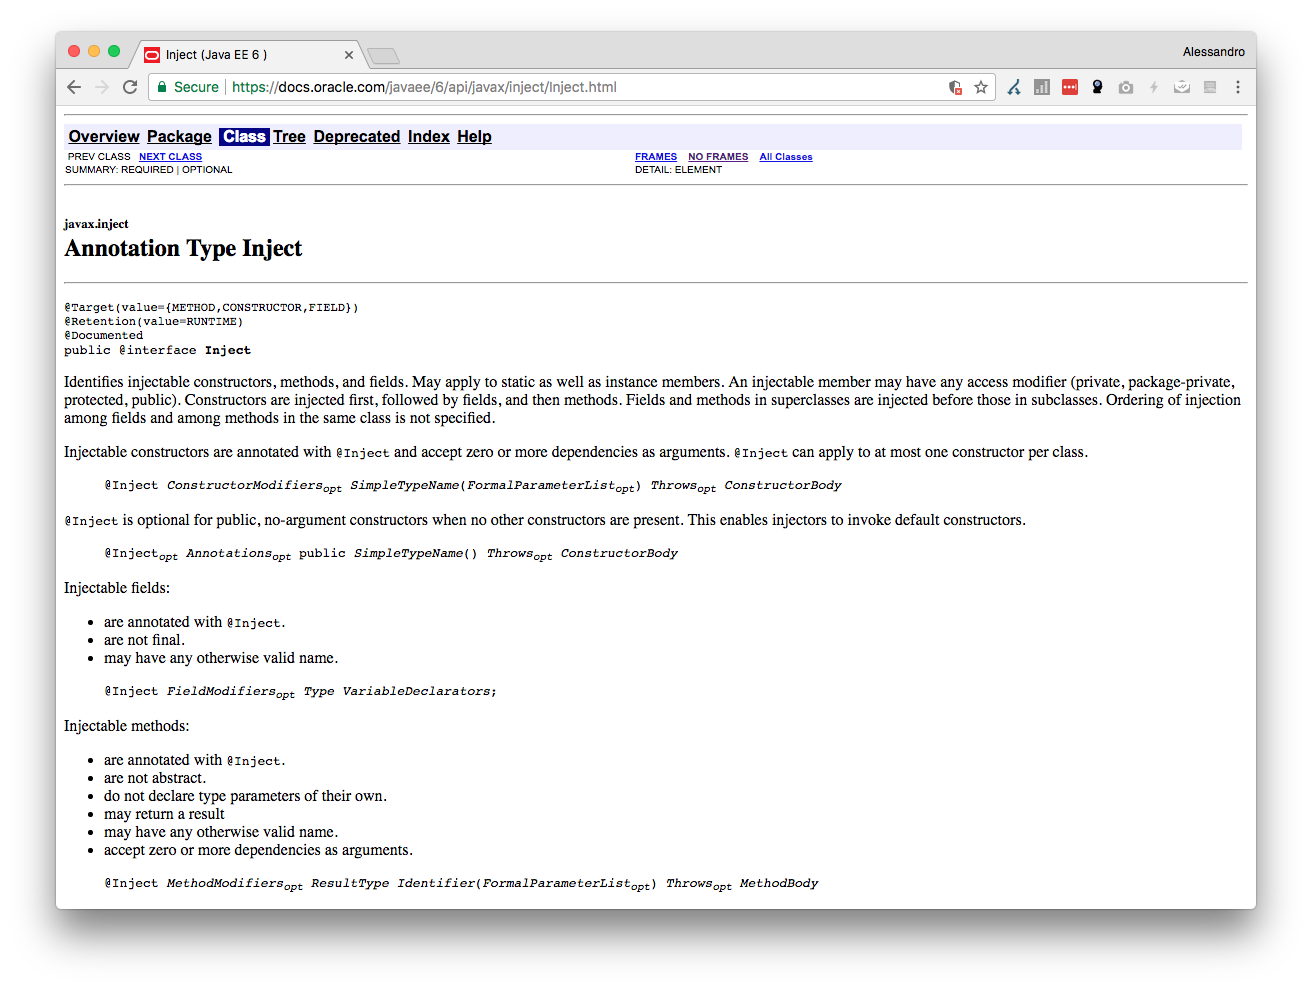
\includegraphics[width=.9\textwidth]{inject}
	\end{figure}
	\url{https://docs.oracle.com/javaee/6/api/javax/inject/Inject.html}
\end{frame}
\begin{frame}[fragile]
\begin{lstlisting}[language=Kotlin, basicstyle=\ttfamily]
// provides the dependencies 
class Module {
    fun providePresenter(): Presenter {
        val okHttp : OkHttp = ...
        val gson : Gson = GsonBuilder = ...
        val retrofit : Retrofit = ...
        val repository : Repository = /*...*/
        val usecase : UseCase = /*...*/
	return Presenter(usecase) 
    }
}
\end{lstlisting} 
\end{frame}
\begin{frame}[fragile]
	We can be more granular:
\begin{lstlisting}[language=Kotlin, basicstyle=\ttfamily]
class Module {
  fun providesOkHttp() : OkHttp = /*..*/
  fun providesGson() : Gson = /*..*/
  fun providesRetrofit(gson:Gson, okHttp : OkHttp) 
       : Retrofit = /*..*/
  fun providesRepository(retrofit : Retrofit) 
       : Repository = /*..*/
  fun providesUseCase(repository:Repository) 
       : UseCase = /*..*/
    
  fun providePresenter(useCase: UseCase) 
       : Presenter = PresenterImpl(usecase) 
}
\end{lstlisting} 
\end{frame}
\begin{frame}
	\begin{itemize}
		\item modules provide a flexible, pluggable, \emph{declarative} definition on how to instantiate dependencies in the modules 
		\item we have just to implement the interface for the injector that builds the necessary dependencies and plug them into the target (wiring) 
	\end{itemize}
\end{frame}
\plain{The end\ldots (really?)}
\begin{frame}[fragile]
	\begin{alertblock}{inconveniences}
		\begin{itemize}
			\item Boilerplate in implementing the injector 
			\item 
		Combinatorial explosion when chaining mutual dependencies
		\end{itemize}
	\end{alertblock}
\end{frame}

\begin{frame}
	Dependency injection frameworks help to \emph{automatic organise} the graph of dependencies. 

	Common DI frameworks for the Java platform:
	\begin{itemize}
		\item Pivotal's Spring Core Container (autowiring) 
		\item Google's Guava 
		\item Square's Dagger1
		\item Google's Dagger2
	\end{itemize}
\end{frame}

\begin{frame}
	Two strategies (common in java):
	\begin{itemize}
		\item Reflection (runtime) 
		\item JSR-269 Annotation processing (compile time)
	\end{itemize}

	Pros/cons\ldots 
\end{frame}

	\section{Dagger2}
	\begin{frame}
		Dagger2 is
		\begin{itemize}
			\item fully static 
			\item compile-time 
			\item annotation processing based 
			\item Java/Android
			\item dependency injection framework
			\item for organising dependencies into a \emph{directed acyclic graph
				}	(DAGger)
		\end{itemize}
	\end{frame}

	\begin{frame}[fragile]
\begin{lstlisting}[language=Kotlin, basicstyle=\ttfamily]
// Gradle module file 
implementation group: 'com.google.dagger', \
        name: 'dagger', \
	version: '2.14.1'
implementation group: 'com.google.dagger', \ // <-- 
     name: 'dagger-compiler', 
     version: '2.14.1'
\end{lstlisting} 
Check 
		\url{https://mvnrepository.com/artifact/com.google.dagger/dagger/}
\end{frame}


	\begin{frame}[fragile]
\begin{lstlisting}[language=Kotlin, basicstyle=\ttfamily]
@Module
class NetworkModule {
  @Provides
  fun providesOkHttp() : OkHttp = /*..*/

  @Provides
  fun providesGson() : Gson = /*..*/

  @Provides 
  fun providesRetrofit(gson:Gson, okHttp : OkHttp) 
       : Retrofit = /*..*/
}
\end{lstlisting} 
\end{frame}

\begin{frame}[fragile]
	\begin{figure}
		\centering
		\includegraphics[width=.9\textwidth]{retrofit_Dagger}
	\end{figure}
\end{frame}

	\begin{frame}[fragile]
\begin{lstlisting}[language=Kotlin, basicstyle=\ttfamily]
@Component(modules = arrayOf(
        ModuleA::class,
        ModuleB::class,
        ModuleC::class
))
interface ApplicationComponent {

	fun inject(activity : MainActivity)
}

\end{lstlisting} 
\end{frame}
	\begin{frame}[fragile]
\begin{lstlisting}[language=Kotlin, basicstyle=\ttfamily]
val applicationComponent = 
   DaggerApplicationComponent.builder() // <--
    .moduleA(ModuleA())
    .moduleB(ModuleB())
    .moduleC(ModuleC())
    .build()
\end{lstlisting} 
\end{frame}

	\begin{frame}[fragile]
		Some dependencies are application-wise (\eg, network or DB). They will be provided through a component rooted at the application level:
\begin{lstlisting}[language=Kotlin, basicstyle=\ttfamily]
class MyApplication : Application() {
  lateinit var component: ApplicationComponent
  override fun onCreate() {
    super.onCreate()
    applicationComponent 
      = DaggerApplicationComponent.builder()
         .moduleA(ModuleA(this))
         .moduleB(ModuleB())
         .moduleC(MOduleC())
         .build()
    }
}
\end{lstlisting} 
\end{frame}
\begin{frame}
	Strategy:
	\begin{itemize}
		\item Avoid relying only on application level components; scope your dependencies (\eg, have other components rooted at activity/fragment classes)
		\item Subcomponents allow to have visibility on higher-component dependencies (\eg, a presenter can see netwok request dependencies) 
		\item Scopes are defined by where the component is rooted (annotations can help identify scoping issues) 
		\item Scopers are not related to android
	\item the purpose of scope annotations is to point Dagger provide either scoped or unscoped objects. But it’s our responsibility  to ``scope''. 
		\item Dependencies are instantiated on-demand if/when needed
	\end{itemize}
\end{frame}
	\begin{frame}[fragile]
\begin{lstlisting}[language=Kotlin, basicstyle=\ttfamily]
@MyActivityScope
@Component(modules = arrayOf(ModuleD::class))
interface MyActivityComponent {
    fun inject(activity: MyActivity)
}

@Scope
@Retention(AnnotationRetention.RUNTIME)
annotation class MyActivityScope
\end{lstlisting} 
		\begin{alertblock}{Warning!}
Module $D$ will not have access to dependencies defined in modules $A$, $B$ and $C$ for application component, because this is a new independent component
		\end{alertblock}
\end{frame}
	\begin{frame}[fragile]
\begin{lstlisting}[language=Kotlin, basicstyle=\ttfamily]
val myActivityComponent = 
   DaggerMyActivityComponent.builder() // <--
    .moduleA(ModuleD())
    .build()
\end{lstlisting} 
\end{frame}
	\begin{frame}[fragile]
\begin{lstlisting}[language=Kotlin, basicstyle=\ttfamily]
class MyActivity : Activity() {
  lateinit var component: MyActivityComponent
  override fun onCreate() {
    super.onCreate()
    component  
      = DaggerMyActivityComponent.builder()
         .moduleA(ModuleD(this))
         .build()
    }
}
\end{lstlisting} 
\end{frame}
\begin{frame}[fragile]
	Subcomponents:
\begin{lstlisting}[language=Kotlin, basicstyle=\ttfamily]
@MyActivityScope
@SubComponent(modules = arrayOf(ModuleD::class))
interface MyActivityComponent {
    fun inject(activity: MyActivity)
}

@Scope
@Retention(AnnotationRetention.RUNTIME)
annotation class MyActivityScope
\end{lstlisting} 
		\begin{alertblock}{Warning!}
This time, Module $D$ will have access to dependencies defined in modules $A$, $B$ and $C$ for application component, because this is a subcomponent
		\end{alertblock}
\end{frame}
	\begin{frame}[fragile]
\begin{lstlisting}[language=Kotlin, basicstyle=\ttfamily]
@Component(modules = arrayOf(
   ModuleA::class,
   ModuleB::class,
   ModuleC::class
))
interface ApplicationComponent {

  fun plus(moduleD : ModuleD) : MyActivityComponent
  fun inject(activity : MainActivity)
}

\end{lstlisting} 
	\end{frame}

\begin{frame}[fragile]
\begin{lstlisting}[language=Kotlin, basicstyle=\ttfamily]
class MyActivity : Activity() {
  lateinit var component: MyActivityComponent
  override fun onCreate() {
    super.onCreate()
    val applicationComponent = /* .... */
    component  = applicationComponent
         .plus(ModuleD(this))
    }
}
\end{lstlisting} 
		\begin{alertblock}{Spoiler!}
This way, MyActivity knows it's injector!  Violation of DI in a strict sense.
		\end{alertblock}
\end{frame}

	\begin{frame}[fragile]
\begin{lstlisting}[language=Kotlin, basicstyle=\ttfamily]
\end{lstlisting} 
\end{frame}
\begin{frame}
	With dagger we can replace (at compilation time) the implementation of some interfaces with
	\begin{itemize}
		\item debug-only variants of the dependencies (\eg, with logs), keeping the app code exactly the same as per production app 
		\item mocked dependencies for java testing (and testing the exact code of the app) 
		\item mocked dependencies for instrumented testing  (\eg, unit test of the view mocking the presenter)  
		\item Easily replace or enhanced (via decorator pattern) the dependencies without impacting changing any other area of the code (as long as the contract of the interface is the same) 
	\end{itemize}
			
\end{frame}
\begin{frame}
	Things to keep in mind:
	\begin{itemize}
		\item if there is an error (\eg, missing dependency) you are not able to build the project (no unexpected issues at runtime), most of the time the error message is informative
		\item Dagger provides no help for dynamic dependency injection at runtime 
		\item Dagger increases compilation time (generation of new java files occurs at compilation time)
		\item If not used carefully, it might instantiate lot of stuff at starting time, leading to slower startup times of the app%
			\footnote{the same can happen manually of course, but sometimes it's easier if dependecies are just handled by dagger2}
	\end{itemize}
\end{frame}

	\section{Dagger2 Android }

\begin{frame}[fragile]
\begin{lstlisting}[language=Kotlin, basicstyle=\ttfamily]
implementation group: 'com.google.dagger', \
               name: 'dagger-android', \
	       version: '2.14.1'

kapt group: 'com.google.dagger', \
     name: 'dagger-android-processor',  \
     version: '2.14.1'
\end{lstlisting} 
\end{frame}

\begin{frame}[fragile]
\begin{lstlisting}[language=Kotlin, basicstyle=\ttfamily]
class MyActivity : AppCompatActivity() {

    @Inject
    lateinit var presenter: Presenter

    override fun onCreate(bundle: Bundle?) {
        AndroidInjection.inject(this) // <--  AMAZING 
        super.onCreate(savedInstanceState)
        setContentView(R.layout.activity_login)
    }
}
\end{lstlisting} 
\end{frame}


\begin{frame}[fragile]
Less amazing stuff here\ldots 
\begin{lstlisting}[language=Kotlin, basicstyle=\ttfamily]
@Module
abstract class ActivityBuilder {
    @ContributesAndroidInjector(modules = arrayOf(ModuleD::class))
    internal abstract fun bind(): MyActivity
}
\end{lstlisting} 
\end{frame}

\begin{frame}[fragile]
\begin{lstlisting}[language=Kotlin, basicstyle=\ttfamily]
@Component.Builder
    interface Builder {

        @BindsInstance
        fun application(application: Application): Builder

        fun build(): ApplicationComponent

    }
\end{lstlisting} 
\end{frame}

\begin{frame}[fragile]
\begin{lstlisting}[language=Kotlin, basicstyle=\ttfamily]
open class MyApplication : Application(), 
               HasActivityInjector {

    @Inject
    lateinit var dispatcher: DispatchingAndroidInjector<Activity>

    override fun onCreate() {
        super.onCreate()
        DaggerApplicationComponent.builder()
                .application(this)
                .build()
                .inject(this)
    }
    override fun activityInjector(): AndroidInjector<Activity>? {
        return activityDispatchingAndroidInjector
    }
}
\end{lstlisting} 
\end{frame}

	\section{Alternative patterns}
	\begin{frame}[fragile]
		\begin{itemize}
			\item Cake pattern
			\item Reader monad 
			\item Implicits (Scala)
		\end{itemize}
	\end{frame}
\plain{Questions?}

%\begin{frame}[allowframebreaks] {References}
% \bibliography{demo}
% \bibliographystyle{abbrv}
%\end{frame}

\end{document}
